\documentclass[10pt,a4paper,twocolumn]{article}
\usepackage[margin=1.8cm,columnsep=0.6cm]{geometry}
\usepackage[T1]{fontenc}
\usepackage{lmodern}
\usepackage{microtype}
\usepackage{booktabs}
\usepackage{tabularx}
\usepackage{graphicx}
\usepackage{enumitem}
\usepackage{xcolor}
\usepackage{amsmath}
\usepackage{caption}
\usepackage[hidelinks]{hyperref}

\setlist{itemsep=1pt,topsep=3pt,leftmargin=*}
\captionsetup{font=small,labelfont=bf}
\newcommand{\src}[1]{\texttt{\footnotesize #1}}
\newcommand{\dec}[1]{\textsf{#1}}
\newcommand{\pos}{\textcolor[HTML]{1baf7a}{\textbf{+}}}
\newcommand{\negr}{\textcolor[HTML]{eb6834}{\textbf{--}}}
\newcommand{\finding}[1]{\par\smallskip\noindent\fbox{\parbox{\dimexpr\linewidth-2\fboxsep-2\fboxrule}{\small #1}}\par\smallskip}

\title{\Large When Does Soft Tissue Matter for Robotic Ultrasound?\\[3pt]
\large A patient-specific deformable simulator, one positive measurement finding,\\ and two negative results}
\author{MTP project --- research status report}
\date{13 November 2026}

\begin{document}
\twocolumn[
\maketitle
\begin{abstract}
\noindent
We extended a SonoGym-style robotic ultrasound gym with patient-specific soft tissue: every one of 13 CT patients
gets a finite-element (FEM) model of skin, fat and muscle, the probe pushes into it with a controlled force, and the
ultrasound (B-mode) image is rendered from the \emph{deformed} anatomy. We then asked one question, with every
hypothesis written down before the run: \emph{what does the deformation actually change?}
The answer so far is narrow but clear.
(1)~\textbf{Measurement: yes.} The paraspinal muscle measured from the image gets thinner as the probe pushes
harder, by $0.25$--$0.30$~mm per newton on two held-out patients, tracking the true compression; a rigid simulator
shows a flat line. (2)~\textbf{Policy behaviour: no.} A navigation policy trained on rigid tissue with the probe
allowed to sink in behaves the same as one trained on deformable tissue (success gap $-0.8$ points). What separates
rigid-trained from deformable-trained policies is the probe's indentation, which any rigid simulator can add.
(3)~\textbf{An off-the-shelf soft-body engine (MuJoCo~4 flex) failed} a pre-registered accuracy and speed gate.
We explain each result in plain language, list the limitations, and lay out what to try next, including other
organs and the runs that need the GPU server.
\end{abstract}
\vspace{1em}]

% =====================================================================================================
\section{Introduction}

\paragraph{The problem in one paragraph.}
A robot holding an ultrasound probe has to press on the patient: without contact there is no image. Pressing
squeezes the soft tissue under the probe. Robot-learning simulators for ultrasound, such as SonoGym~\cite{sonogym},
treat the body as rigid: the probe is placed on the skin, and the image is a slice through an undeformed CT. If the
squeezing matters, policies trained in such simulators may learn the wrong thing. If it does not matter, rigid
simulators are good enough and are much cheaper. Nobody has measured which is true, on real patient anatomy.

\paragraph{What we built.} A GPU gym (\src{mtp\_gym}) with the same patients and similar tasks as SonoGym, plus:
\begin{itemize}
  \item a patient-specific linear FEM of the soft tissue, solved for all parallel environments at once;
  \item a force controller, so the probe presses with a target force (typically 4~N) and the indentation depends on
    the patient's anatomy;
  \item an ultrasound simulator that renders the image from the \emph{deformed} CT;
  \item three tissue modes that let us separate causes (Fig.~\ref{fig:modes}):
    \textbf{rigid} (SonoGym-style, probe on the skin),
    \textbf{kinematic} (probe pressed in, tissue not deformed) and
    \textbf{deformable} (probe pressed in, tissue deformed);
  \item a live bridge to 3D Slicer and a 1~kHz robot physics loop (PyBullet or MuJoCo).
\end{itemize}

\paragraph{How we test.} Every study is \emph{pre-registered}: the hypothesis, the metric, the pass/fail threshold
and the analysis script are committed to git before the run (\src{DECISIONS.md}, entries \dec{DEC-0xx}).
Negative results are reported, not re-run with relaxed thresholds. Every number below comes from a file in
\src{results/} whose name is given next to it.

\paragraph{What we found.}
\begin{itemize}
  \item[\pos] Deformation changes a clinical \emph{measurement} (muscle thickness) in a way a rigid simulator cannot
    reproduce (\S\ref{sec:thick}).
  \item[\negr] Deformation does not change \emph{policy behaviour} in navigation; the probe's indentation does
    (\S\ref{sec:nav}).
  \item[\negr] Deformation does not change rigid-bone reconstruction, the force--image trade-off hypothesis failed,
    and learned policies do not yet generalise to new patients (\S\ref{sec:earlier}).
  \item[\negr] MuJoCo~4's soft bodies are either inaccurate or about 380 times too slow for this use
    (\S\ref{sec:mujoco}).
\end{itemize}
The short version: \textbf{soft tissue matters when the thing you measure is the soft tissue itself, and does not
matter (yet) when the robot only has to find a rigid landmark at a fixed force.}

% =====================================================================================================
\section{Background}
\begin{itemize}
  \item \textbf{SonoGym}~\cite{sonogym} offers robotic-ultrasound learning tasks (navigation to a standard view of
    the L4 vertebra, bone surface reconstruction) on CT patients from TotalSegmentator~\cite{totalseg}. Its
    anatomy is rigid and its contact force is not simulated.
  \item \textbf{CRESSim-Neo}~\cite{cressim} has a batched GPU soft-body ultrasound scanning environment, but no
    patient CT anatomy and no fidelity check of the tissue model against a reference.
  \item \textbf{Clinical muscle thickness.} Paraspinal (lumbar multifidus/erector) thickness is measured with
    ultrasound in back-pain research as the distance from the thoracolumbar fascia to the facet joint~\cite{thu}.
    Probe pressure is a known nuisance in such measurements; a simulator can quantify it per patient.
\end{itemize}

% =====================================================================================================
\section{The simulator}
\label{sec:sim}

\begin{figure*}[t]
\centering
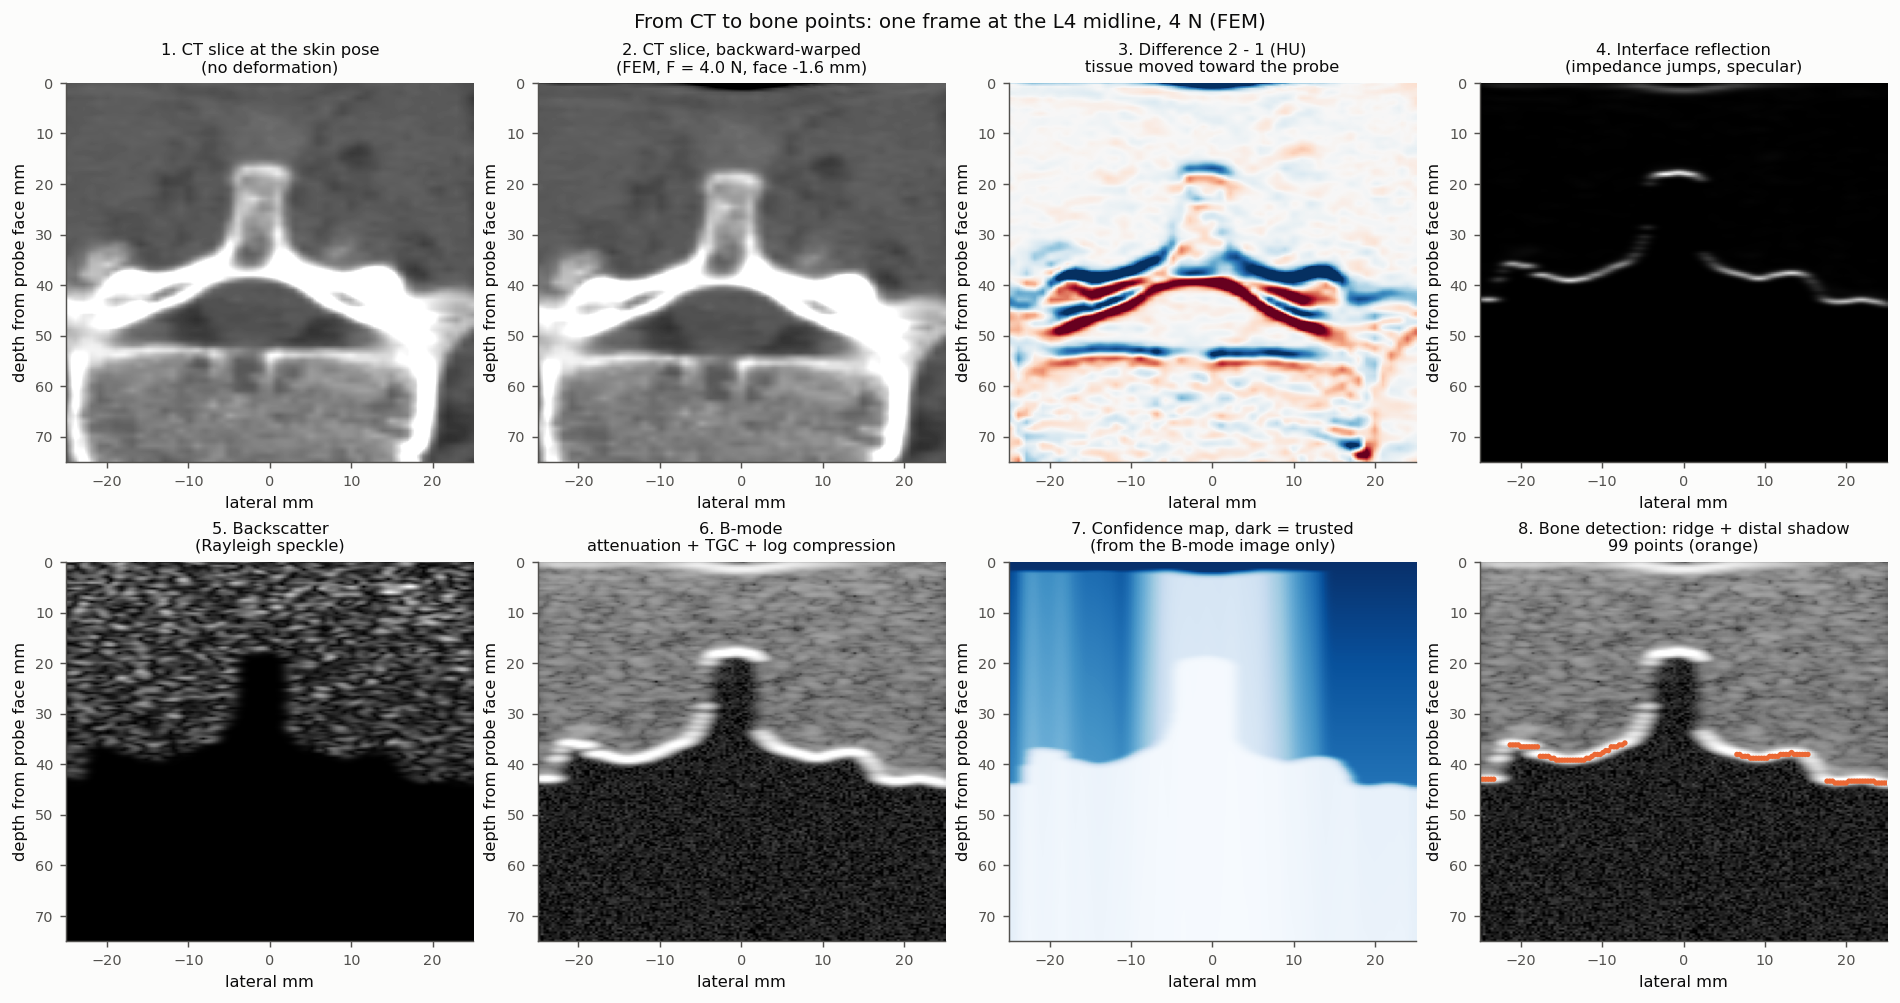
\includegraphics[width=\linewidth]{fig_bmode_pipeline.png}
\caption{\textbf{From CT to image, one frame (illustration).} (1)~CT slice at the skin pose; (2)~the same slice
pulled through the FEM displacement at 4~N; (3)~their difference (tissue moves towards the probe); (4)--(6)~the
ultrasound physics (reflections at tissue interfaces, speckle, attenuation, fixed gain); (7)--(8)~the image-only
bone detector. Made on 5~Nov by \src{ReconstructionPipeline/scripts/make\_soft\_body\_report.py}; it uses the earlier
B-mode settings, before the depth physics of \dec{DEC-042/043} made deep tissue darker.}
\label{fig:pipeline}
\end{figure*}

\paragraph{Anatomy.} 13 patients: the 12 TotalSegmentator subjects SonoGym uses plus one sample patient. The split
is 9 training and 4 held-out patients, stratified by tissue thickness (\src{data/splits.json}). Skin, fat, muscle and
bone come from the segmentation labels.

\paragraph{Soft tissue.} A linear tetrahedral FEM per patient (4~mm elements), with the bone held fixed. The
expensive part (the tissue's response to a push) is precomputed once per patient, so each query is cheap and runs
on the GPU for all environments together (\dec{DEC-041}). Intuitively, the model knows in advance ``how this back
gives way when pushed here'', and only has to combine those responses at run time. Fig.~\ref{fig:deform} shows a
push at 4 and 8~N.

\begin{figure}[t]
\centering
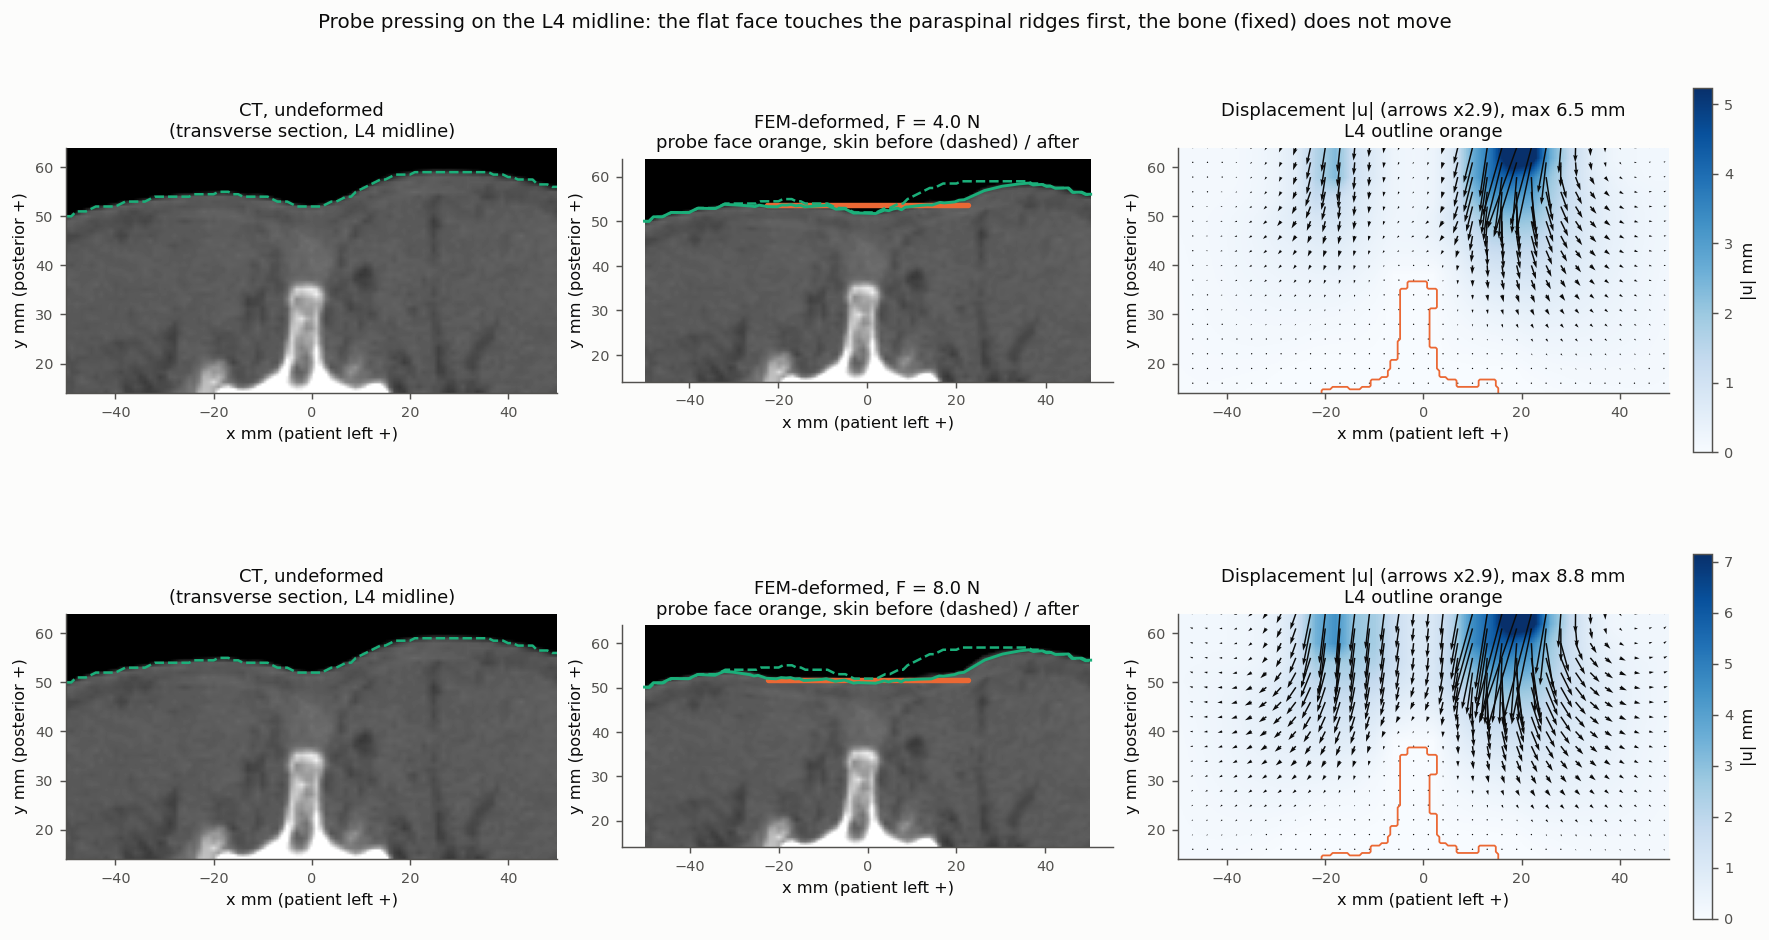
\includegraphics[width=\linewidth]{fig_deformation_field.png}
\caption{\textbf{The FEM at work (illustration).} Transverse CT through the L4 midline. Left: undeformed. Middle: the
flat probe face (orange) pushes the skin down; dashed is the skin before. Right: displacement field; the bone (outline)
does not move. Top 4~N, bottom 8~N. Made on 5~Nov, after the contact model of \dec{DEC-040}.}
\label{fig:deform}
\end{figure}

\paragraph{Is the linear FEM accurate?} We compared it with a large-strain (Neo-Hookean) reference solver on 3
patients, 2 sites and 4 forces (\dec{DEC-047}). At 2~N the linear model's compression is within $-4.9$ to $+1.8$\,\%
of the reference (median $-1.3$\,\%); at 5--15~N errors reach about $\pm 30$\,\%
(\src{results/fem\_fidelity\_20261107\_234638}). \emph{So the FEM is trustworthy up to about 5~N}, which is why the
studies below treat 1--5~N as primary and report higher forces separately.

\paragraph{Ultrasound image.} Model-based, from the (deformed) CT: attenuation per tissue, reflection and
transmission at interfaces, speckle, a fixed time-gain compensation, and (since \dec{DEC-055}) a 1.65~mm
thoracolumbar fascia layer with literature properties~\cite{pirri,miles}. The fascia matters: without it the muscle's
upper boundary was invisible in the image and the muscle could not be measured at all (\dec{DEC-051}).

\paragraph{Speed.} The batched gym runs 530 environment-steps/s with deformable tissue at 32 environments on the
laptop RTX~2050 (665 rigid; \src{results/throughput\_20261105\_235332}). With PPO learning on top, a 300k-step
navigation run takes 40--53~min (95--125 steps/s; training metadata in \src{checkpoints/vec\_ppo/nav\_*.json}).

\paragraph{Robot side.} A 1~kHz physics loop runs in its own process with a Franka Panda, PyBullet by default or
MuJoCo~3 (\dec{DEC-052}); both hold 1000.0~Hz on a quiet machine
(\src{results/physics\_rate\_20261112\_125735\_idle\_post\_review.json}). The scene streams to 3D Slicer over
OpenIGTLink, including the deformed skin and the live B-mode (Fig.~\ref{fig:flexdemo}). The robot's own compliance
is \emph{not} fed back into the tissue or the image.

\begin{figure*}[t]
\centering
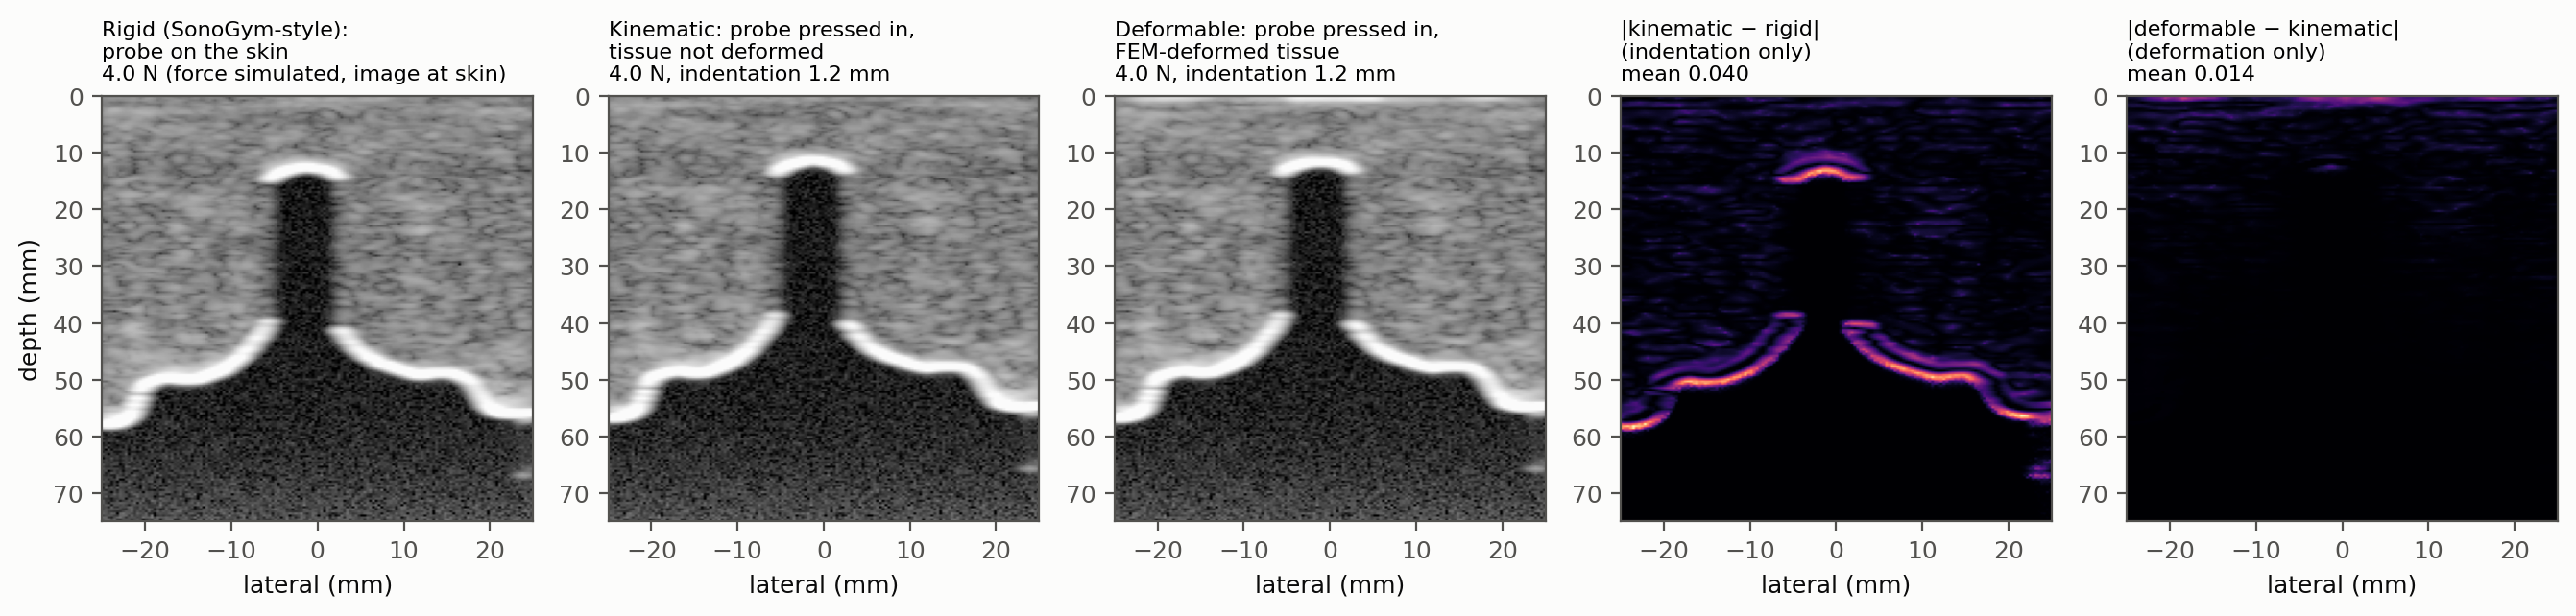
\includegraphics[width=\linewidth]{fig_demo_modes.png}
\caption{\textbf{The three tissue modes, same patient (s0015, training set) and probe pose, 4~N (illustration).}
Rigid (SonoGym-style) images at the skin. Kinematic presses the probe 1.2~mm in, but the tissue is not deformed.
Deformable presses it in and warps the tissue. Right: what changes between them. Indentation shifts every echo,
including the bone (mean absolute difference 0.040); the deformation itself mostly changes the first millimetres
under the probe (0.014). Rendered by \src{make\_figures.py} at the current commit; one speckle seed. The test
\src{test\_kinematic\_mode\_presses\_into\_rigid\_tissue} gives 0.011 vs 0.068 at another pose on the sample patient.}
\label{fig:modes}
\end{figure*}

% =====================================================================================================
\section{Result 1: soft tissue changes a measurement}
\label{sec:thick}

\paragraph{Question (\dec{DEC-056}, pre-registered).} When the probe pushes harder, does the paraspinal muscle
thickness \emph{read from the image} shrink as the real muscle does, and does a rigid simulator miss it?

\paragraph{Set-up.}
\begin{itemize}
  \item Thickness = fascia to bone, the clinical definition~\cite{thu}. The image measurement uses the B-mode
    only: the fascia echo above and the bone echo below. The ground truth uses the warped segmentation labels and is
    never shown to the detector.
  \item 6 sites per patient, forces 1, 2, 3, 4, 5~N (8 and 10~N reported only).
  \item Two conditions at the same pressed-in probe pose: deformable tissue, and rigid tissue (kinematic).
  \item The detector was tuned on training patients only and frozen before the held-out patients were run.
  \item A site counts only if the muscle is not cut off by the 75~mm image window and the bone is visible
    (\dec{DEC-054}). This leaves 2 of the 4 held-out patients measurable.
\end{itemize}

\begin{figure}[t]
\centering
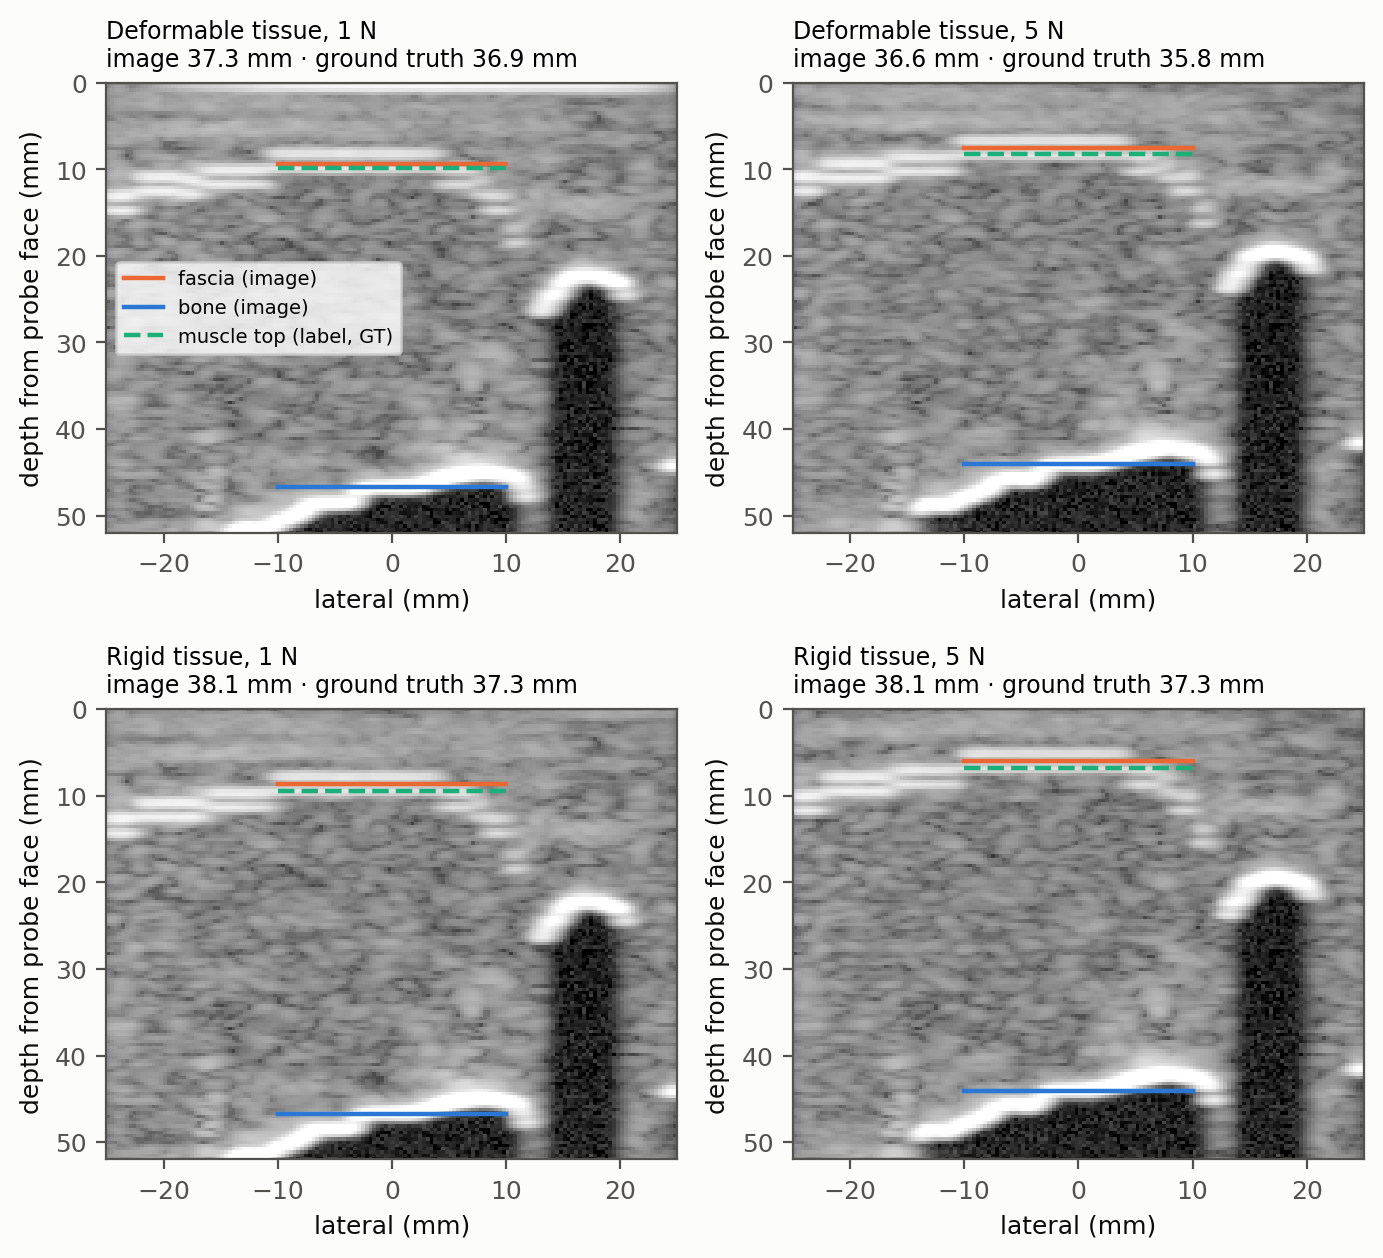
\includegraphics[width=\linewidth]{fig_demo_muscle.png}
\caption{\textbf{What the measurement sees (illustration; training patient s0015, one site).} Orange: fascia found
in the image; blue: bone found in the image; dashed green: true muscle top. From 1 to 5~N, the deformable image's
thickness drops (37.3$\to$36.6~mm; truth 36.9$\to$35.8). In rigid tissue the whole picture moves up because the probe
sinks in, but the thickness stays at 38.1~mm: \emph{nothing gets squeezed}.}
\label{fig:muscle}
\end{figure}

\begin{figure}[t]
\centering
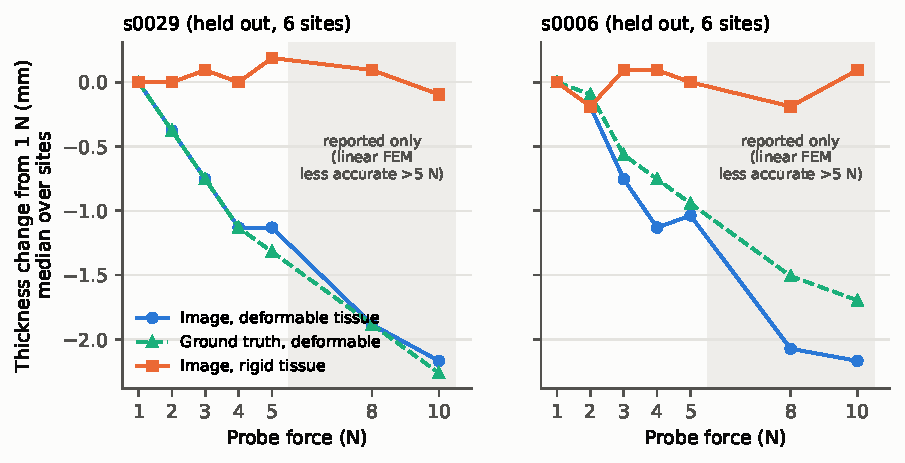
\includegraphics[width=\linewidth]{fig_thickness_vs_force.pdf}
\caption{\textbf{Result 1.} Change in measured thickness from 1~N, median over sites, for the two measurable
held-out patients. The image (blue) follows the truth (green) in deformable tissue; the rigid simulator (orange) stays
flat. Source \src{results/muscle\_thickness\_20261112\_151349.json}.}
\label{fig:thick}
\end{figure}

\begin{table}[t]
\centering\footnotesize
\begin{tabular}{@{}lccc@{}}
\toprule
 & s0029 & s0006 & Criterion \\
\midrule
Detection at $\le$2~N & 1.00 & 1.00 & median $\ge 0.5$ \\
$|$image $-$ truth$|$ at $\le$2~N (mm) & 0.75 & 2.26 & median $< 3$ \\
Image slope, deformable (mm/N) & $-0.302$ & $-0.245$ & $< 0$ \\
True slope, deformable (mm/N) & $-0.339$ & $-0.226$ & --- \\
Image slope, rigid (mm/N) & $+0.019$ & $+0.038$ & $|\cdot| \le 0.15$ \\
\midrule
\multicolumn{4}{@{}l}{G (measurable) \textbf{pass}: detection 1.00, error 1.51~mm}\\
\multicolumn{4}{@{}l}{H4 (tracks compression, rigid flat) \textbf{pass}: tracking gap 0.075~mm/N}\\
\multicolumn{4}{@{}l}{H5 (force-aware correction helps) \textbf{fail}: 1.31 vs 1.32~mm}\\
\bottomrule
\end{tabular}
\caption{Thread B v2 on the held-out patients (slopes over 1--5~N, 6 sites each). s0034 is not measurable (detection
0.00) and s0030 has no site inside the image window. Source \src{results/muscle\_thickness\_20261112\_151349.md}.}
\label{tab:thick}
\end{table}

\paragraph{Result.} Gates G and H4 pass (Table~\ref{tab:thick}, Fig.~\ref{fig:thick}). The image-measured muscle
thins by $0.25$--$0.30$~mm per newton, within 0.075~mm/N of the truth, while the rigid simulator's measurement stays
within $\pm 0.04$~mm/N of zero. Over 1--5~N this is about 1--1.3~mm, a few percent of a 35--40~mm muscle.

\paragraph{Why H5 failed, intuitively.} H5 asked whether a single correction ``add $k$~mm per newton'', learned on
training patients, makes held-out measurements more accurate. It does not (1.31 vs 1.32~mm; uncorrected 0.75~mm).
The constant offset between image and truth differs from site to site by about as much as the whole force effect, so
a population-wide correction removes the wrong amount. Within a site the slope is real; across sites it is drowned
out.

\finding{\textbf{Take-away 1.} A rigid simulator reports the same muscle thickness at any probe force; the deformable
one reports thinner muscle at higher force, as a real one would. This is a property a rigid gym cannot have, measured
on held-out patients. It is small (about 1~mm over 1--5~N) and rests on 2 measurable patients.}

% =====================================================================================================
\section{Result 2: soft tissue does not change navigation behaviour}
\label{sec:nav}

\paragraph{Question (\dec{DEC-057}, pre-registered).} Does a navigation policy behave differently depending on the
tissue model it was trained on? If yes, modelling policy outcomes is worth it; if no, not for this task.

\paragraph{Set-up.} Task: move the probe to the standard L4 view, with the patient's position hidden from the
policy~(\dec{DEC-045}). PPO, 300k steps, 2 training patients, 2 seeds per condition, trained in each of the three
modes of Fig.~\ref{fig:modes}. Every policy is then tested in every mode on the same 2 patients (64 episodes each).
\begin{itemize}
  \item \emph{SonoGym gap} = deformable-trained minus rigid-trained success, tested on deformable tissue.
  \item \emph{Deformation-only gap} = deformable-trained minus kinematic-trained success, tested on deformable
    tissue. This is the one that says whether the \emph{deformation} matters.
  \item A gap counts if its mean is $\ge 15$ points and both seeds agree in sign. Rule: move on to policy outcomes
    only if the deformation-only gap counts.
\end{itemize}

\begin{table}[t]
\centering\footnotesize
\begin{tabular}{@{}lccc@{}}
\toprule
Trained \textbackslash{} tested on & deformable & kinematic & rigid \\
\midrule
deformable, seed 0 & 0.984 & 0.984 & 0.734 \\
deformable, seed 1 & 1.000 & 1.000 & 0.953 \\
kinematic, seed 0 & 1.000 & 1.000 & 0.906 \\
kinematic, seed 1 & 1.000 & 1.000 & 0.812 \\
rigid, seed 0 & 0.797 & 0.750 & 1.000 \\
rigid, seed 1 & 0.953 & 0.922 & 1.000 \\
\midrule
oracle / blind / random & \multicolumn{3}{c}{1.000 / 0.094 / 0.062 (all modes)} \\
\midrule
\multicolumn{4}{@{}l}{Deformation-only gap: $-1.6$, $0.0$ (mean $-0.8$) --- does not count}\\
\multicolumn{4}{@{}l}{SonoGym gap: $+18.8$, $+4.7$ (mean $+11.7$) --- does not count}\\
\bottomrule
\end{tabular}
\caption{Navigation success, training mode $\times$ test mode. Source \src{results/nav\_transfer\_20261112\_183531.md}.}
\label{tab:nav}
\end{table}

\begin{figure}[t]
\centering
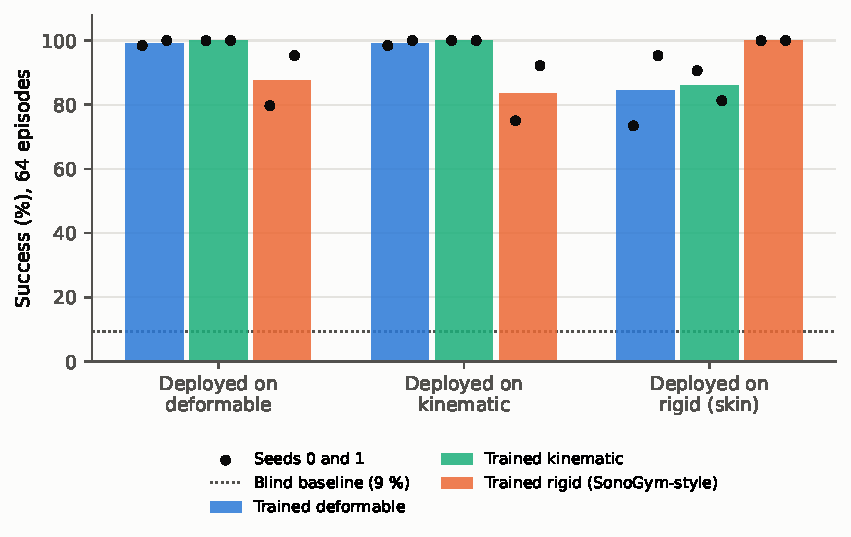
\includegraphics[width=\linewidth]{fig_nav_transfer.pdf}
\caption{\textbf{Result 2.} Bars: mean of the two seeds; dots: each seed. Deformable- and kinematic-trained policies
are indistinguishable everywhere. Rigid-trained policies lose ground on both pressed-in modes alike, so their loss
comes from the indentation, not the deformation. Same source as Table~\ref{tab:nav}.}
\label{fig:nav}
\end{figure}

\paragraph{Result.} Neither gap counts (Table~\ref{tab:nav}, Fig.~\ref{fig:nav}); by the pre-registered rule we do
not model policy outcomes for navigation. Three observations explain it:
\begin{itemize}
  \item \textbf{Kinematic = deformable, everywhere.} Same success (0.98--1.00), same final error (1.2--2.0~mm), same
    episode length (5--6 steps).
  \item \textbf{The indentation is what matters.} Rigid-trained policies drop about as much on kinematic tissue
    (no warp) as on deformable tissue. Pressing the probe in shifts every echo by the indentation
    (Fig.~\ref{fig:modes}); a rigid simulator can add that by letting the probe sink in.
  \item \textbf{Navigation cannot show a deformation effect as designed.} The force is held at 4~N by the controller
    and the policy cannot change it (mean force 3.97--4.00~N for all policies), so the warp is a small, constant
    change near the skin. Kinematic and deformable policies are also already at the ceiling (98--100\,\%).
\end{itemize}

\finding{\textbf{Take-away 2.} For finding a bony landmark at a fixed force, a rigid simulator with an indented probe
trains policies that are as good as a deformable one. This is a useful negative result for anyone choosing a
simulator, but it is not a reason to use soft tissue.}

% =====================================================================================================
\section{Earlier results, positive and negative}
\label{sec:earlier}

\begin{table*}[t]
\centering\footnotesize
\begin{tabularx}{\linewidth}{@{}p{3.1cm}Xp{4.6cm}@{}}
\toprule
Study & Result, in plain terms & Source (\src{results/}) \\
\midrule
\pos~Force needs anatomy & The same indentation takes 9.43~N on a thin back and 3.48~N on a thick one: force
  and indentation are patient-specific. & test \src{test\_anatomy\_changes\_force\_under\_shared\_moduli} (\dec{DEC-041}) \\
\pos~FEM accuracy & Within 5\,\% of a large-strain reference at 2~N; up to $\pm 30$\,\% at 5--15~N. &
  \src{fem\_fidelity\_20261107\_234638} \\
\pos~Imaging depends on fat & With depth physics, mean bone coverage over 13 patients drops 0.659$\to$0.376 and falls
  with paraspinal fat (Spearman $\rho=-0.79$). & \src{bmode\_physics\_compare\_20261107\_190506} \\
\pos~Force decides what is visible & Thick back s0014: bone visible at 0 of 9 poses at 1~N and 8 of 9 at 15~N. Works
  through indentation. & \src{compression\_sweep\_20261105\_235841} \\
\pos~Benchmark validity & A blind policy solved navigation from the pose alone until the patient offset was hidden;
  the area reward paid for wandering until replaced by coverage gain. & \dec{DEC-045}, \dec{DEC-046} \\
\negr~Reconstruction & For a rigid bone and a tracked probe, deformation does not change reconstruction: coverage
  88.0 vs 88.8\,\%. & \dec{DEC-048} \\
\negr~Force vs image (H2) & Pre-registered: the best force would differ between thin and thick backs. It does not
  (2~N for both). & \dec{DEC-042}, \dec{DEC-044} \\
\negr~Echo shift & The bone echo shift under force is the same with and without the warp (deformation part 0.00~mm in
  11 of 12 patients): it is probe kinematics. Earlier claim withdrawn. & \src{kinematic\_vs\_deformation\_20261108\_020955} \\
\negr~Generalisation & Navigation: 100\,\% on training patients, at most 14.1\,\% on held-out patients for any training set
  or augmentation (blind 3.1\,\%). & \src{vec\_eval\_nav\_20261108\_075931} \\
\negr~Reconstruction PPO & Does not beat random on held-out patients (0.32--0.34 vs 0.34; raster 0.43). &
  \src{vec\_eval\_recon\_20261108\_020410} \\
\bottomrule
\end{tabularx}
\caption{Results from 5--8 November. Green plus: supports the simulator or a finding; orange minus: negative.}
\label{tab:earlier}
\end{table*}

Table~\ref{tab:earlier} lists the other results. The pattern is the same as in Results~1 and~2: wherever the
target is \emph{bone} (which does not deform) the soft tissue's effect reduces to how far the probe sinks in, which
is kinematics. The one place deformation matters is a \emph{soft} target.

% =====================================================================================================
\section{Result 3: MuJoCo soft bodies fail the gate}
\label{sec:mujoco}

MuJoCo~4 (released 6 Nov 2026) has native soft bodies (\emph{flex}). We tested whether it could replace or improve
our FEM, against a gate written before the study (\dec{DEC-053}): every case within 10\,\% of the large-strain
reference at 2--5~N; no worse than the linear FEM at 10--15~N; no inverted elements; a re-settle within 33~ms.

\begin{table}[t]
\centering\footnotesize
\begin{tabularx}{\linewidth}{@{}lXX@{}}
\toprule
 & SVK (default) & Stable Neo-Hookean \\
\midrule
Error at 2~N & 90--420\,\% & 1.2--4.5\,\% \\
Worst at 2--5~N & --- & $+15.1$\,\% (one 5~N case) \\
Median at 10--15~N & 252\,\% (linear: 15\,\%) & 18.8\,\% (linear: 14.9\,\%) \\
Inverted elements & all 24 cases & 7 of 24 cases \\
Time per re-settle & 50.5~s & 12.5~s (budget 33~ms) \\
\midrule
Passes & no & no \\
\bottomrule
\end{tabularx}
\caption{MuJoCo flex gate, same mesh, moduli and nodal forces as the reference. Source
\src{results/mujoco\_flex\_fidelity\_20261112\_112537.md}.}
\label{tab:flex}
\end{table}

\begin{figure}[t]
\centering
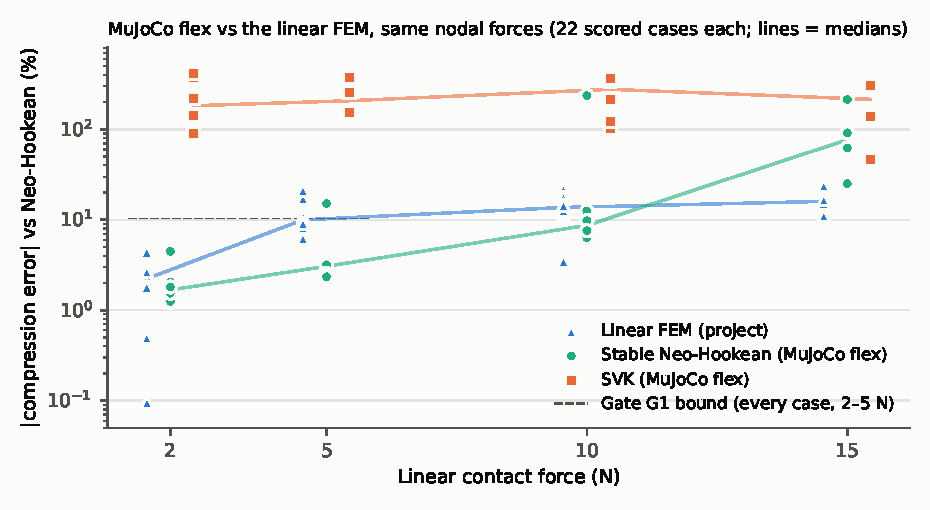
\includegraphics[width=\linewidth]{fig_flex_gate.pdf}
\caption{Compression error vs the Neo-Hookean reference, per case (log scale). Same source as
Table~\ref{tab:flex}.}
\end{figure}

\paragraph{Why, intuitively.} (i)~The default SVK material is known to go soft and turn elements inside out under
strong compression; the few skin nodes under the probe are strongly compressed even at 2~N. (ii)~Stable Neo-Hookean
is accurate at small strain but is not the same energy as our reference, so they part at large strain. (iii)~Speed is
structural: MuJoCo time-steps the whole mesh until it comes to rest, while our FEM answers from precomputed responses.
At 2--5~N, where the good material is accurate, our linear FEM is already within about 5\,\%.

\begin{figure*}[t]
\centering
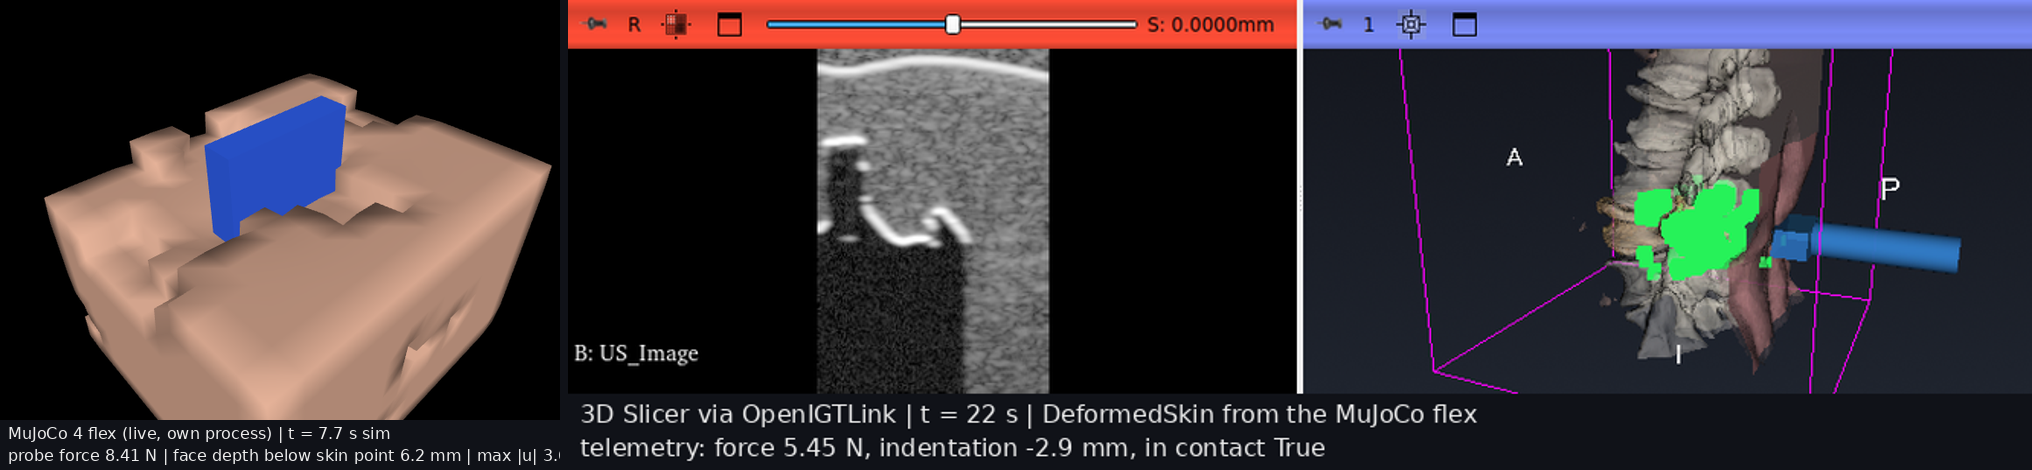
\includegraphics[width=\linewidth]{fig_demo_flex.png}
\caption{\textbf{MuJoCo flex demonstration (demo only, not a validated tissue model).} Left: the live MuJoCo~4
flex patch of the patient mesh (Stable Neo-Hookean) pressed by the probe, in its own process. Middle and right: 3D
Slicer receiving the deformation and the B-mode over OpenIGTLink while the robot scans. Recorded on 13 Nov with
\src{scripts/demo\_mujoco\_flex\_slicer.sh}; the force and depth in the captions are read from the run's CSV logs.}
\label{fig:flexdemo}
\end{figure*}

\finding{\textbf{Take-away 3.} An off-the-shelf soft-body engine is either wrong from first contact or about 380
times over the time budget for interactive, quasi-static tissue. What remains useful is MuJoCo as the
\emph{robot} engine: a compliant, torque-controlled arm that holds 1~kHz.}

% =====================================================================================================
\section{Discussion: what the results add up to}

\begin{table}[t]
\centering\footnotesize
\begin{tabularx}{\linewidth}{@{}Xc@{}}
\toprule
Statement & Status \\
\midrule
A batched, patient-specific deformable US gym exists and runs at laptop scale & \pos \\
Its tissue model is accurate (within 5\,\%) up to $\sim$5~N & \pos \\
Deformation changes a soft-tissue measurement; rigid sims cannot & \pos \\
Required force and imaging difficulty are patient-specific & \pos \\
Deformation changes rigid-bone reconstruction & \negr \\
Deformation changes navigation behaviour & \negr \\
Learned policies generalise to new patients & \negr \\
An off-the-shelf soft-body engine can replace the FEM & \negr \\
Any of this holds on real patients or phantoms & untested \\
\bottomrule
\end{tabularx}
\caption{Ledger of claims.}
\end{table}

\paragraph{A simple rule that fits every result.} Deformation can only change an outcome if two things are true:
\begin{enumerate}
  \item \textbf{the target itself is soft} (it moves or changes size under the probe), and
  \item \textbf{the outcome depends on that change by more than the measurement noise}.
\end{enumerate}
Bone fails (1). Muscle thickness passes both, but only just: about 1~mm of compression against 0.75--2.26~mm of
per-patient error. Navigation at a fixed force fails both: the target is bone, and the policy cannot vary the force.

\paragraph{What we can claim honestly.}
\begin{itemize}
  \item A soft-tissue robotic-US gym on SonoGym's patients with a validated force range.
  \item Where soft tissue matters: measurement of soft structures.
  \item Where it does not: navigation to bony views, and reconstruction of bone; there a rigid simulator with
    indentation is enough. This negative result is useful for the field: it tells simulator builders where to spend
    effort.
\end{itemize}

% =====================================================================================================
\section{Limitations}
\begin{itemize}
  \item \textbf{No real data.} Nothing is compared with real ultrasound, a phantom or a robot. All findings are
    simulator findings.
  \item \textbf{Tissue parameters.} All patients share the same moduli. The fat modulus (11~kPa) is higher than the
    1--2~kPa a literature search reported (not yet verified). No per-patient stiffness.
  \item \textbf{Tissue physics.} Linear, quasi-static, frictionless contact; accurate only up to $\sim$5~N. No
    organ sliding, no breathing, no fluid. The robot's compliance does not feed back into the tissue.
  \item \textbf{Anatomy.} CTs are supine; ultrasound of the back is done prone. The fascia is a synthetic layer placed
    at the muscle label's edge, with literature properties.
  \item \textbf{Imaging.} The image is derived from CT intensity on a compressed impedance scale; no reverberation
    or clutter. An earlier audit found the simulator easier than real ultrasound.
  \item \textbf{Statistics.} Result~1 rests on 2 measurable held-out patients, 6 sites each, one speckle seed.
    Result~2 uses 2 patients, 2 seeds and 300k steps, and its policies are at the ceiling. One held-out patient
    (s0006) was looked at during the fascia check before the study; this is disclosed in \dec{DEC-056}.
  \item \textbf{Generalisation.} No learned policy works on new patients yet (at most 14\,\%), so policy results hold
    for training patients only.
\end{itemize}

% =====================================================================================================
\section{Open directions}
\label{sec:open}

\paragraph{A. Write up what we have.} Results 1--3 plus the simulator are complete and pre-registered. Framing:
``where soft tissue matters for robotic ultrasound, and where it does not''.

\paragraph{B. A task where the policy chooses the force.} For example: measure the muscle thickness, scored
against the uncompressed truth. A rigid-trained policy is never penalised for pressing hard, so it should press
harder and measure thinner muscle. Risk: Result~1 already predicts this without RL (about 0.3~mm/N, so about 0.9~mm
from 1 to 4~N), and force-scan PPO did not beat random at laptop scale.

\paragraph{C. A softer organ, where the target moves.} The rule above says to look for targets that are soft and
whose motion is large compared with the image error. The abdomen is the natural candidate: TotalSegmentator already
labels liver, kidneys, spleen, the major vessels and more~\cite{totalseg}, so the same pipeline applies. Candidate
tasks:
\begin{itemize}
  \item \textbf{Liver lesion or vessel targeting} (e.g. for biopsy or ablation guidance): the target moves under the
    probe, so a policy trained on rigid anatomy would aim at the wrong place.
  \item \textbf{Vessel compressibility}: in venous compression ultrasound, whether a vein collapses under the probe
    is itself the diagnostic sign. Deformation \emph{is} the outcome. It needs a model of a fluid-filled, collapsing
    vessel, which a linear FEM cannot provide.
  \item \textbf{Organ size measurements} (kidney, liver span) under probe pressure, the abdominal analogue of
    Result~1.
\end{itemize}
New problems the abdomen brings: organs slide against each other, breathing moves them by more than the probe
does, ribs and bowel gas block the view, and the tissue moves far beyond the linear FEM's 5~N comfort zone. Stiffness
values must come from elastography literature, checked before use.

\paragraph{D. Close the generalisation gap (thread A).} The original primary thread. It needs many more patients
and much longer training than the laptop allows (below).

\paragraph{E. A real-data anchor.} Even one phantom with a known stiffness, scanned by hand at several forces, would
test Result~1 outside the simulator and remove the largest limitation.

% =====================================================================================================
\section{What to run on the GPU server}
\label{sec:server}

The laptop GPU has 4~GB and holds about 3 patients; a 300k-step navigation run takes 40--53~min. The workstation
(RTX~5000-class, to be confirmed) is reachable only from the institute network. Planned runs, each to be
pre-registered before it starts:

\begin{table}[h]
\centering\footnotesize
\begin{tabularx}{\linewidth}{@{}Xp{2.6cm}@{}}
\toprule
Run & Unlocks \\
\midrule
Download TotalSegmentator v2 (23.6~GB) and build FEM assets for many more patients & everything below; more
measurable patients for Result~1 \\
Result~1 on tens of held-out patients (cheap: no training) & a real confidence interval for the 0.3~mm/N effect \\
Navigation with 4, 9 and more training patients, 3+ seeds, millions of steps, with and without FEM augmentation &
thread A (H1--H3); whether the held-out gap closes \\
Direction B: force-choosing measurement task at scale & a policy-level soft-tissue effect, if one exists \\
Per-patient large-strain (Neo-Hookean) precompute and stiffness randomisation & forces above 5~N; per-patient
stiffness \\
Direction C pilot: liver/abdomen meshes and FEM precompute for a few patients & whether the organ switch is
feasible \\
\bottomrule
\end{tabularx}
\caption{Server workload. Run times on the server are not yet measured; the laptop figures above are the only
measured basis.}
\end{table}

% =====================================================================================================
\section{Conclusion}
We built a patient-specific soft-tissue extension of a robotic ultrasound gym, validated its tissue model in its
working range, and asked where deformation matters. Pre-registered tests give one positive answer (soft-tissue
measurement) and several negative ones (bone reconstruction, navigation, an off-the-shelf soft-body engine). The
negative results are informative: for bony targets at a fixed force, a rigid simulator with indentation is enough.
The next decisions are whether to publish this map as it stands, to find a task where the policy's force choice
matters, or to move to a softer organ where targets move under the probe.

\begin{thebibliography}{9}\footnotesize
\bibitem{sonogym} SonoGym: a benchmark for robotic ultrasound. arXiv:2507.01152, 2025.
\bibitem{cressim} CRESSim-Neo. arXiv:2608.25192, 2026.
\bibitem{totalseg} J.~Wasserthal \emph{et al.} TotalSegmentator: robust segmentation of 104 anatomic structures in CT
  images. \emph{Radiology: Artificial Intelligence}, 2023.
\bibitem{thu} Thu \emph{et al.} \emph{Journal of Pain Research} 15:1457--1463, 2022.
\bibitem{pirri} C.~Pirri \emph{et al.} \emph{Diagnostics} 13:1436, 2023.
\bibitem{miles} C.~A.~Miles. \emph{J.\ Acoust.\ Soc.\ Am.} 99:3225, 1996.
\end{thebibliography}

\onecolumn
\appendix
\section{Reproducing every number and figure}
\small
\begin{tabularx}{\linewidth}{@{}lX@{}}
\toprule
Item & Command or file \\
\midrule
Result 1 & \src{./.venv/bin/python ReconstructionPipeline/evaluation/muscle\_thickness\_study.py}, then
  \src{muscle\_thickness\_analysis.py results/muscle\_thickness\_<stamp>.json} \\
Result 2 & \src{bash scripts/run\_nav\_transfer.sh} (about 3~h on the laptop) \\
Result 3 & \src{./.venv/bin/python ReconstructionPipeline/evaluation/mujoco\_flex\_fidelity.py} \\
Figures & \src{./.venv/bin/python Docs/reports/research\_2026-11-13/make\_figures.py} (data figures from
  \src{results/}; illustrations rendered at the current commit) \\
MuJoCo demo & \src{bash scripts/demo\_mujoco\_flex\_slicer.sh --seconds 40} \\
Videos & \src{demonstrations/demo\_fem\_soft\_body.mp4}, \src{demonstrations/report/reconstruction\_raster\_fem.mp4},
  \src{demonstrations/report/tilt\_shear\_fem.mp4} \\
Decisions & \src{DECISIONS.md}: \dec{DEC-041} to \dec{DEC-057} \\
Branch & \src{thread-b-muscle}; test suite on 13 Nov: 214 passed, 3 expected failures (known limitations, strict) \\
\bottomrule
\end{tabularx}
\end{document}
